\subsection{Protein Synthesis}
The last process of the central dogma -- the translation of RNA into protein
-- is the final subject in our dialogue between back-of-the-envelope
estimates and comparison with proteomic data. Here we consider the number of
ribosomes needed to replicate the cellular proteome. While the rate at which
ribosomes translates is well known to have a growth rate dependence
\citep{dai2018}, here we make the approximation that translation occurs at a
rate of $\approx$ 15 amino acids per second per ribosome (BNID: 100233).
Under this approximation and assuming a division time of 5000 s, we can
easily arrive at an estimate of $\approx 10^4$ ribosomes needed to replicate
the entire protein mass (\FIG{protein_synthesis}). This point estimate and
the corresponding estimate across a continuum of growth rates proves to be
notably comparable to the experimental observations, shown in
\FIG{protein_synthesis}(B). While the ribosome is responsible for the
formation of peptide bonds, we do not diminish the importance of the charging
of tRNAs with the appropriate amino acid, a process with occurs with
remarkable accuracy. In the Appendix and in
\FIGSUPP[protein_synthesis]{tRNA}, we consider the process of ligating tRNAs
to their corresponding amino acid and again find notable comparability with
the data.

Having now completed our circuit through key processes of cellular growth
outlined in \FIG{categories}, we can now take stock on our understanding of the
observed growth rate dependence and abundances of various protein complexes. We
note that in general, these simple estimates have been reasonably successful in
quantitatively describing the observations in the proteomic data, suggesting
that the proteome is tuned in composition and absolute abundance to match the
growth rate requirements, without any one process representing a particular
bottleneck or rate limiting step in division. However, in our effort to identify
key limitations on growth, there are two notable observations that we wish to
emphasize.

The first is a recurring theme throughout our estimates, which is that any
inherent biochemical rate limitation can be overcome by expressing more
proteins. We can view this as a parallelization of each biosynthesis task,
and this helps explain why bacteria tend to increase their protein content (and
cell size) as they grow faster \citep{ojkic2019}. The second, and ultimately
the most significant in defining the cellular growth rate, is that the
synthesis of ribosomal proteins presents a special case where parallelization
is \textit{not} possible and thereby imposes a limit on the fastest possible
growth rate. This presents an optimization problem for
the cell -- how are the translational demands of the entire proteome met without
investing resources in producing an excess of ribosomes?



% The need for ribosomes to replicate themselves leads us to
% propose that translation is a primary determinant of growth.
% With a typical translation rate of $\approx$ 15 AA per second and
% $\approx$ 7500 amino acids in a ribosome, each ribosome requires $\approx$ 7
% minutes to be synthesized [\cite{dill2011}, \FIG{ribosome_limit}(A)]. Thus, for
% \textit{E. coli} this serves as a hard lower bound for the rate at which
% division could occur, predicted on the assumption that division is dependent
% only on the ability to replicate the cellular ribosomal pool. In reality,
% however, cells are tasked with replicating their entire proteome and not
% \textit{just} the ribosomal fraction.

This question, more frequently presented as a question of optimal resource
allocation, has been the target of an extensive dialogue between experiment and
phenomenological modeling over the past decade. In a now seminal work,
\cite{scott2010} presents an elegant treatment of resource allocation through
partitioning of the proteome into sectors -- one of which being
ribosome-associated proteins -- the relative sizes of which ultimately define
the total cellular growth rate. In more recent years, this view has been more
thoroughly dissected both experimentally and theoretically
\citep{klumpp2014,basan2015,dai2018, dai2016, erickson2017} and together
represent a paradigm-shift in how we think of cellular physiology at the
proteome-level. However, the quantitative description of the observations is
often couched in terms of phenomenological constants and effective parameters
with the key observable features of expression being computed in relative rather
than absolute abundances. Furthermore, these approaches often exclude or
integrate away effects of cell size and chromosome content, which we have
illustrated in our estimates to have deep connections to the observed cellular
growth rate.

In the closing sections of this work, we explore how ribosome content, cell
size, and chromosome content are intertwined in their control over the cellular
growth rate. To do so, we take a more detailed view of ribosome abundance,
exchanging our order-of-magnitude estimates for a minimal mathematical model of
growth rate control, defined by parameters with tangible connections to the
biological processes underlying cellular growth. Using this model, we
interrogate how the size of the ribosome pool and its corresponding activity is
regulated to balance the supply of amino acids via metabolism and catabolism
with consumption of amino acids through peptide bond formation.

%While this is a critical step
%in protein synthesis whose efficiency reflects the nutritional richness of the
%growth medium, the ability to parallelize this process by expressing more tRNA
%ligases makes it unlikely to be a bottleneck for cell division.


% We will begin our exploration of protein translation in the same spirit as in
% previous sections with an estimate of the number of ribosomes needed to
% replicate the proteome.
% Ribosomes are enormous
% protein/rRNA complexes that facilitate the peptide bond formation between amino
% acids in the correct sequence as defined by the coding mRNA. Before we examine
% the synthesis of the ribosome proteins and the limits that may place on the
% observed bacterial growth rates, let's consider replication of the cellular
% proteome.
% is a topic which we discuss in detail in
% the coming sections. However, for the purposes of our order-of-magnitude
% estimate, we can
% , while
% glossing over important details such as chromosome copy number and
% growth-rate dependent translation rates,

\begin{figure}
    \centering{
        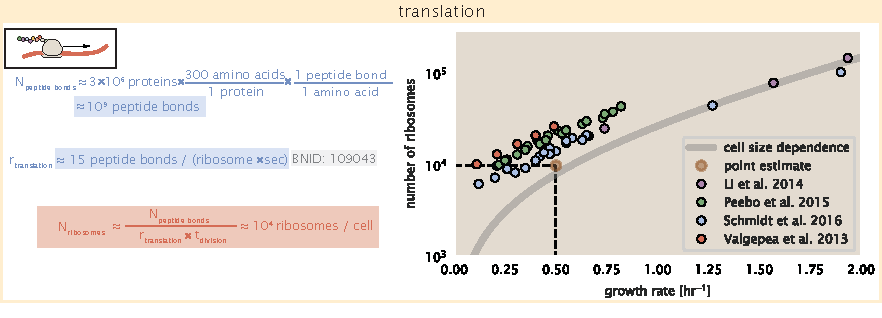
\includegraphics{main_figs/protein_synthesis_main.pdf}
    }
        \caption{\textbf{Estimation of the required number of ribosomes.} Estimation of the
        number of ribosomes required to synthesize 10$^9$ peptide bonds with an
        elongation rate of 15 peptide bonds per second. The
        average abundance of ribosomes is plotted as a function of growth rate.
        Our estimated values are shown for a growth rate of 0.5 hr$^{-1}$.
        Grey lines correspond to the estimated complex abundance calculated at
        different growth rates.} \label{fig:protein_synthesis}

        \figsupp[Estimate and observed abundance and growth rate dependence
        of tRNA ligases.]{Estimation for the number of tRNA synthetases that
        will supply the required amino acid demand. The sum of all tRNA
        synthetases copy numbers are plotted as a function of growth rate
        ([ArgS], [CysS], [GlnS], [GltX], [IleS], [LeuS], [ValS], [AlaS]$_2$,
        [AsnS]$_2$, [AspS]$_2$, [TyrS]$_2$, [TrpS]$_2$, [ThrS]$_2$,
        [SerS]$_2$, [ProS]$_2$, [PheS]$_2$[PheT]$_2$, [MetG]$_2$,
        [lysS]$_2$, [HisS]$_2$, [GlyS]$_2$[GlyQ]$_2$).}{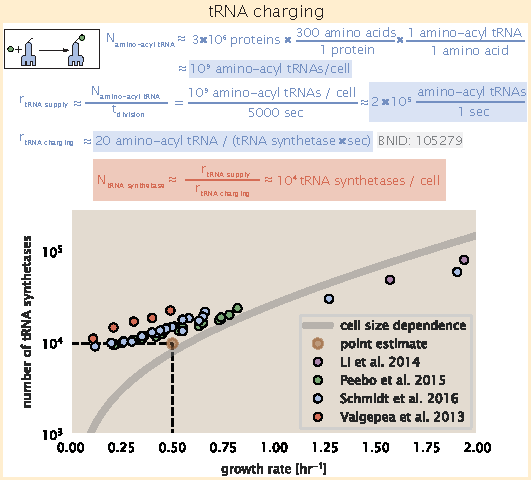
\includegraphics{main_figs/tRNA.pdf}}\label{figsupp:tRNA}
\end{figure}
